\documentclass{article}
\usepackage{amsmath,amssymb}
\usepackage[numbers]{natbib}
\usepackage{geometry}
 \geometry{
 a4paper,
 total={170mm,257mm},
 left=30mm,
 top=30mm,
 right=30mm,
 bottom=30mm
 }
\usepackage{graphicx}
\usepackage{multirow}
\usepackage{siunitx}
\usepackage{booktabs}
\usepackage{gensymb}
\usepackage{float}
\graphicspath{ {../tmp/} }

\setlength{\parskip}{1em}

\title{Reinforcement Learning Assignment-1}
\begin{document}
\author{Utkarsh Prakash \\ \normalsize 180030042}
\maketitle
\begin{enumerate}
    \item Histogram obtained after sampling $N=100$ samples:
        \begin{figure}[H]
            \begin{center}
            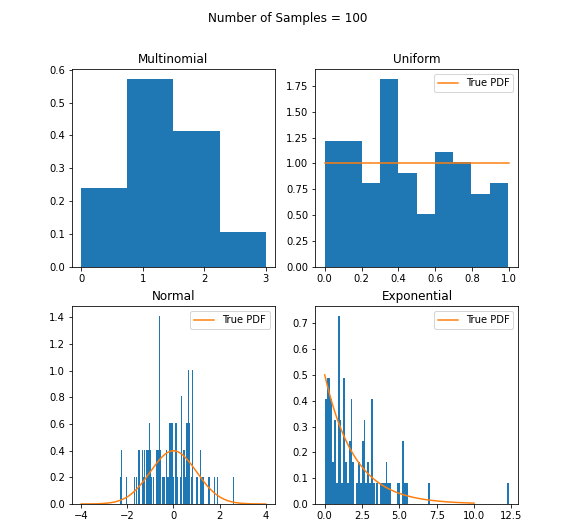
\includegraphics[width=10cm]{Q1_100.png}
            \end{center}
            \caption{Histogram obtained after sampling $N=100$ samples.}
        \end{figure}

        Histogram obtained after sampling $N=1000$ samples:
        \begin{figure}[H]
            \begin{center}
            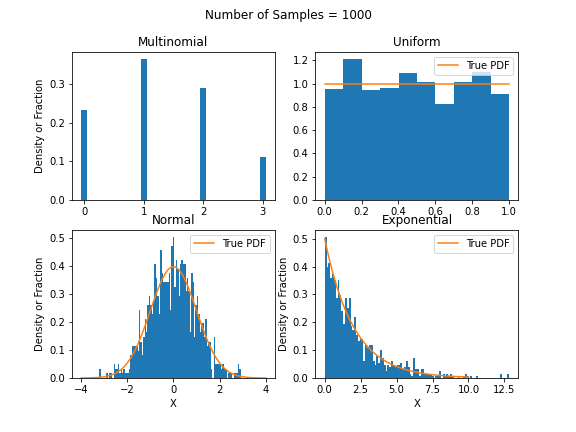
\includegraphics[width=10cm]{Q1_1000.png}
            \end{center}
            \caption{Histogram obtained after sampling $N=1000$ samples.}
        \end{figure}

        Histogram obtained after sampling $N=10000$ samples:
        \begin{figure}[H]
            \begin{center}
            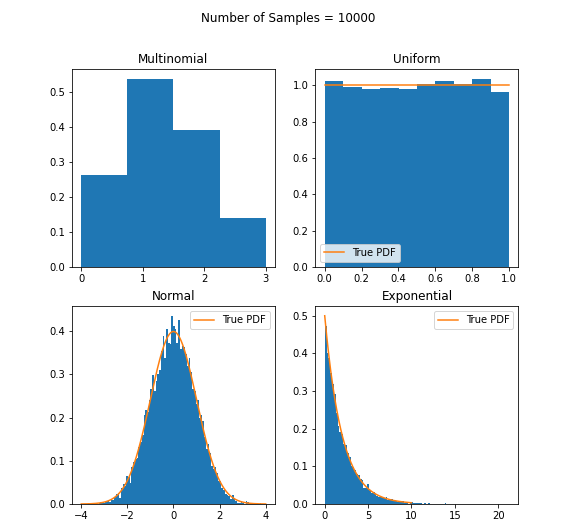
\includegraphics[width=10cm]{Q1_10000.png}
            \end{center}
            \caption{Histogram obtained after sampling $N=10000$ samples.}
        \end{figure}

    \item Let $U \stackrel{}{\sim} Unif(0, 1)$ and $\Phi(x)$ denote the standard normal CDF. Then, we can show that if $X = \Phi^{-1}(U)$,
    then $X \stackrel{}{\sim} \mathcal{N}(0, 1)$. This is because $P(X \le t) = P(\Phi^{-1}(U) \le t) = P(U \le \Phi(t)) = \Phi(t)$. Now,
    since the CDF X is $\Phi(x)$, hence, $X \stackrel{}{\sim} \mathcal{N}(0, 1)$. \par
	
	\noindent %The next paragraph is not indented
    Let $u$ be a sample from $Unif(0, 1)$. Then using the above fact, we generate samples standard normal random samples as 
    $x =\Phi^{-1}(u)$. Then, to generate normal samples with mean $\mu$ and variance $\sigma^{2}$ we can simply transform as 
    $y = \sigma x + \mu$, where $y$ is the sample from normal random variable with mean $\mu$ and variance $\sigma^{2}$.

    \item \textbf{Idea:} In order to compute the integral numerically, we can represent the integration as an expectation of a random 
    variable. Then using Law of Large Numbers, we can compute the expectation, by sampling from the distribution of that random variable.\par
	
	\noindent %The next paragraph is not indented
    Let's $X \stackrel{}{\sim} Unif(0, \pi)$ and $f(x)$ be it's PDF i.e.,
    \begin{equation}
    \nonumber
    f(x) = \begin{cases}
        \frac{1}{\pi} & if 0 \le x \le \pi \\
        0 & otherwise
    \end{cases}
    \end{equation} 
        \begin{enumerate}
            \item Let $g(X) = \sqrt(sin(X))$, where $X$ is as defined above. Then 
                \begin{equation}
                    \mathbb{E}[g(X)] = \int_{-\infty}^{\infty}g(x)f(x) \,dx =  \frac{1}{\pi}\int_{0}^{\pi}g(x) \,dx
                \end{equation}
                Let $X_{1}, X_{2}, ..., X_{N} \stackrel{i.i.d.}{\sim}$ Unif$(0, \pi)$ and $Y_{i} = g(X_{i})$ for $i \in {1, 2, ... N}$. 
                Then according to Law of Large Numbers, we have 
                \begin{equation}
                    \nonumber
                    \lim_{N\to\infty} \frac{1}{N}\sum_{i=1}^{N}Y_{i} = \mathbb{E}[g(X)]
                \end{equation}
                Now,
                \begin{equation}
                    \int_{0}^{\pi}\sqrt(sin(x)) \,dx =  \pi \left ( \lim_{N\to\infty} \frac{1}{N}\sum_{i=1}^{N}Y_{i} \right )
                \end{equation}

            \item We can follow the same thing as above but by defining $g(X) = \sqrt(sin(X))exp(-x^{2})$. 
        \end{enumerate}

\end{enumerate}
\end{document}